\begin{figure}[t]
\centering
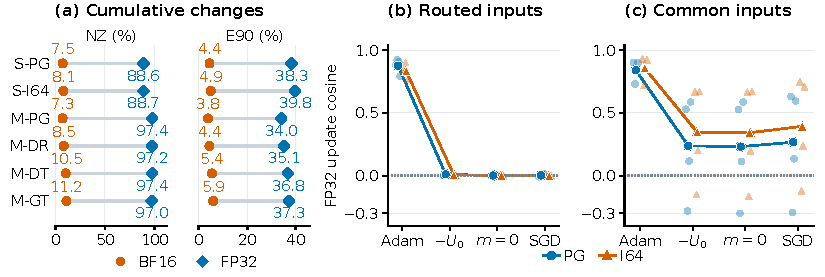
\includegraphics[width=\linewidth]{figures/layout_followup_20260918/section4_sparsity_overlap.pdf}
\caption{\textbf{BF16 rounding hides widespread parameter changes, and shared Adam moments align teacher-specific steps.}
(a) Fractions of changed coordinates (NZ) and coordinates carrying 90\% of squared change (E90), measured in FP32 and BF16.
(b,c) Update cosines on domain-specific/shared inputs; $-U_0$ subtracts the zero-gradient step and $m=0$ resets the first moment. Small/large points show batch/overall means. S/M denote mathematics-only/joint training and PG/I64 denote sampled-token/top-64 supervision. M-DR/DT/GT use top-64 with response/within-domain token/global token averaging; other rows use response averaging.}
\label{fig:subnetwork_overview}
\end{figure}
